\chapter{Clean Architecture}

Zum implementieren der Clean Architecture wurde ein UML Diagramm erstellt (Abb.~\ref{Abb:CleanArchitectureBEFORE} im Anhang) um die aktuellen Abhängigkeiten zu sehen, dabei wurden ein paar Abhängigkeitspfeile weggelassen welche von weit außen nach innen gehen und die Lesbarkeit zu sehr verringern. 


Für die Struktur der Clean Architektur wurde sich auf 4 Schichten festgelegt, da die Funktionsweise des Programms recht simpel ist. Die innerste Schicht beinhaltet alle Entitäten welche zur strukturierten Datenspeicherung verwendet werden. Die mittlere hellblaue Schicht umfasst die Anwendungslogik. Die äußere dunkelgrüne Schicht beinhaltet die Interaktion mit allem Außerhalb, d.h. die Controller zum lesen und schreiben der Daten auf der Festplatte sowie zum kommunizieren mit der GUI. Ganz außen befinden sich die Speicherorte der Spieldaten und die GUI Elemente. 


\begin{figure}[!ht]
  \centering
  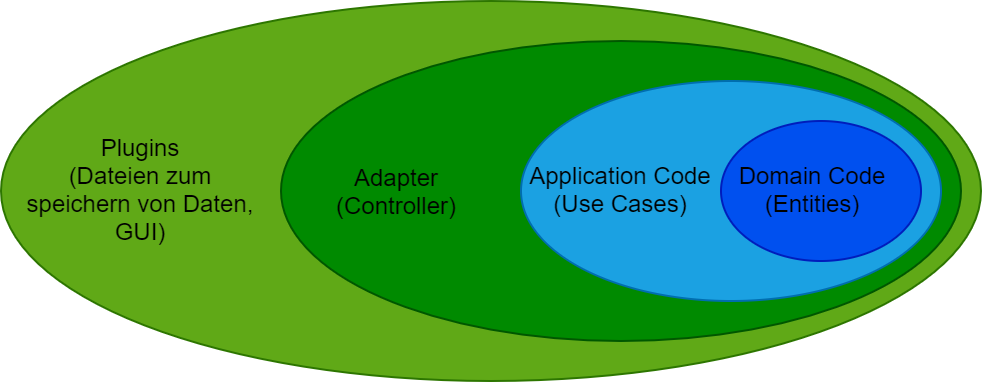
\includegraphics[width=0.6\textwidth]{Bilder/ArchitekturSchichten.PNG}
  \caption{Aufbau der Schichten der Clean Architecture in der Anwendung}
  \label{Abb:ArchitekturSchichten}
\end{figure}

Ein großes Problem sind hierbei Abhängigkeiten von Innen nach Außen, wie z.B. die \textit{WordFinder} Klasse (generiert alle möglichen Buchstabenkombinationen in einem Spielfeld), welche direkt auf den \textit{DataController} (nutzt die Wortliste auf der Festplatte) zugreift, siehe.~\ref{Abb:CleanArchitectureBEFORE} auf Seite~\pageref{Abb:CleanArchitectureBEFORE}. Die Abhängigkeit wird durch Dependency Inversion, d.h. die Erstellung eines Interfaces welches von der äußeren Klasse implementiert und von der inneren genutzt wird, umgedreht \href{https://github.com/EinToni/Wortfinder/commit/586681478211a26abc661239ecc2c297ef77041e}{(Siehe Commit 586681478211a26abc661239ecc2c297ef77041e)}:
\newpage
\begin{figure}[!ht]
  \centering
  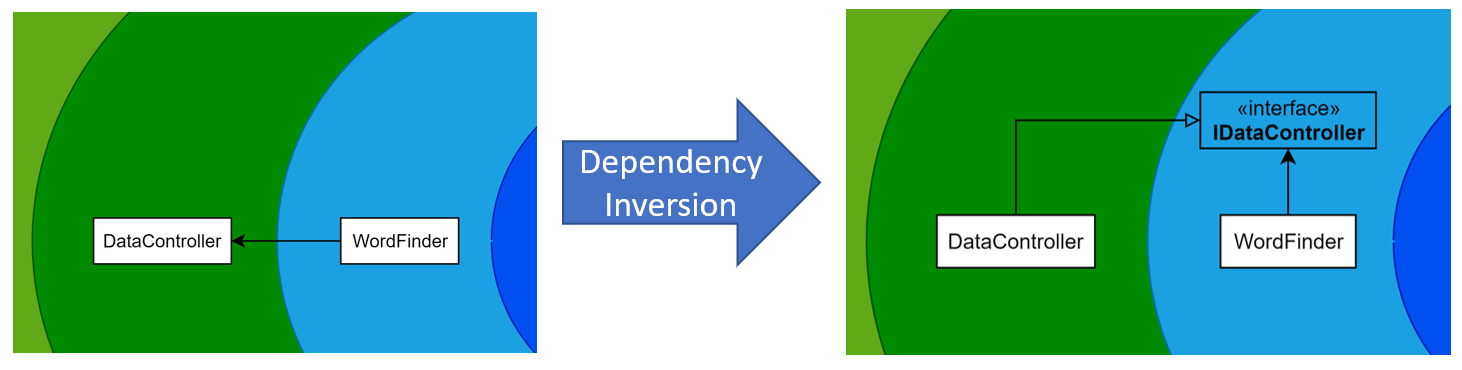
\includegraphics[width=0.8\textwidth]{Bilder/DependencyInversion.PNG}
  \caption{Beispiel der Dependency Inversion}
  \label{Abb:DependencyInversion}
\end{figure}

Wenn innere Klassen äußere erzeugen müssen, wie es beim \textit{WordFinder} der Fall ist, wird das Erzeugungsmuster der abstrakten Fabrik verwendet. Dem \textit{WordFinder} wird dann im Konstruktor eine Referenz auf die Fabrik gegeben. Über die Funktion \glqq GetDataController()\grqq{} gibt die Fabrik dann eine neue Instanz des \textit{DataController} zurück, wobei der Rückgabetyp im Interface der Fabrik als \textit{IDataController} Deklariert ist \href{https://github.com/EinToni/Wortfinder/commit/26148d6a7ae6784b935a260371672fe16f8bbfa0}{vgl. Commit 26148d6a7ae6784b935a260371672fe16f8bbfa0}:

\begin{figure}[!ht]
  \centering
  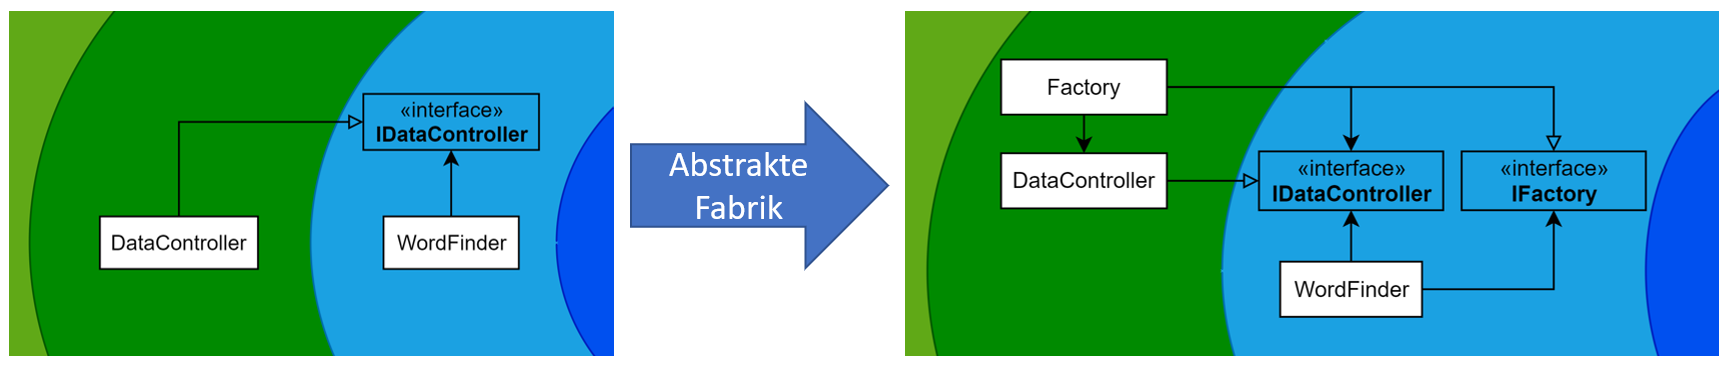
\includegraphics[width=0.8\textwidth]{Bilder/AbstrakteFabrik.PNG}
  \caption{Implementierung der abstrakten Fabrik}
  \label{Abb:AbstrakteFabrik}
\end{figure}

Außerdem problematisch ist der grundsätzliche Aufbau des Programms, sowie speziell der Aufbau des Hauptfensters. Dieses bestand aus einem Grid welches durch den \textit{FieldGenerator} mit Teilfenstern (\textit{LetterBox}, zeigen die Buchstaben an) gefüllt wurde. Jeder \textit{LetterBox} wurde die Instanz des \textit{WordBuilder} gegeben, welchen sie aufrufen wenn sie angeklickt werden.


Zur Verbesserung der Trennung zwischen dem Application Code und der GUI, wird das Grid direkt im Code Behind des \textit{MainWindow} durch kaskadieren von speziellen WPF  Elementen aufgebaut. Die Ansteuerung des \textit{MainWindow} erfolgt dann über einen neuen \textit{MainWindowController} dem im Aufruf nur die Größe des Spielfelds und die Buchstaben übergeben werden. Somit erfolgt die Erstellung der GUI separiert vom restlichen Anwendungscode.


Vor der Implementierung wurde zuerst das erstellte UML Diagramm abgeändert. Zuerst wurde dabei die Stuktur geändert, dann alle Abhängigkeitspfeile welche nach außen zeigen mittels Dependency Inversion umgedreht und als letztes an notwendigen Stellen eine Abstrakte Fabrik hinzugefügt. Das daraus entstandene Diagramm ist im Anhang als Abbildung~\ref{Abb:CleanArchitectureAFTER}.


Mit diesen Vorgaben wurde das Diagramm umstrukturiert, sodass alle Klassen an ihrem sinnvollsten Ort sind. Da das Programm vorher ständig mit Funktionen ergänzt wurde bei denen lediglich Wert auf Funktionalität gelegt wurde, sind im Nachhinein betrachtet unnötig komplizierte Strukturen entstanden. Diese werden daher bei der Umstrukturierung des Diagramms zur Clean Architecture auch gleich geändert. 
%% Beispiel für 
Ein Beispiel hierfür ist die \textit{FindableWords} Klasse, welche alle im aktuelle laufenden Spiel findbaren Wörter beinhaltet. Diese wurde erst später hinzugefügt, da davor direkt jedes vom Nutzer markierte Wort im heruntergeladenen Wörterbuch überprüft wurde. Sowie die \textit{GameGrid} Klasse, welche (unter anderem) die Größe und Buchstaben des Spielfelds beinhaltet. Die findbaren Wörter sowie die Buchstaben im aktuellen Spiel wurden in eine neue Klasse \textit{Game} verschoben welche alle Daten über Spiel enthält. Somit können Spiele auch im Vorhinein generiert und dann geladen werden.


Da Klassenreferenzen teilweise sehr weit an nachfolgende Klassen \glqq weitergereicht\grqq{} werden, wurde die Erstellung aller Klassen und deren Dependency Injection in die Main verschoben. Dadurch wird das unschöne und unübersichtliche weiterreichen vermieden, sowie das Mocken von Klassen ermöglicht welche nun nicht mehr im Konstruktor der jeweiligen Klasse erzeugt, sondern in der Main injiziert werden. Außerdem können die abstrakten Fabriken hierdurch auch wieder entfernt werden, da alle Klassen direkt in der Main erzeugt werden. Der Commit in welchem alle Initialisierungen in die Main ausgelagert wurde und somit die Implementierung der Clean Architecture abgeschlossen ist, ist: \href{https://github.com/EinToni/Wortfinder/commit/15e467c93903dac44e916c61f76792d385abd087}{15e467c93903dac44e916c61f76792d385abd087}. Das sich hieraus ergebende Klassendiagramm ist im Anhang~\ref{Abb:CleanArchitectureAFTERinMain} und online \href{https://github.com/EinToni/WortfinderDoku/blob/main/Bilder/CleanArchitectureAFTERinMain.png}{hier}.


\paragraph{Nachträgliche Korrektur}
Nicht eingehalten wurde die Clean Architecture bei der \textit{WebScraper} und \textit{WordMissingWindow} Klasse. Denn zum Zeitpunkt des Commits war geplant diese nicht mehr zu verwenden und später zu entfernen. Da sie allerdings in Zukunft doch noch verwendet werden sollen, wurden sie, sowie weitere zugehörige Klassen, im Nachhinein korrekt angepasst. Das Klassendiagramm nach welchem die Implementierung durchgeführt wurde ist nachfolgend zu abgebildet. Zu beachten ist allerdings, dass nur die Struktur und die GUI implementiert wurden. Für die korrekte Funktionalität des WebScrapers fehlte allerdings die Zeit. Diese soll aber in Zukunft online im Duden nach betroffene Wort nachschlagen und prüfen ob es existiert. Commit der Implementierung: \href{https://github.com/EinToni/Wortfinder/commit/163a14f0730bb69c9805b4ee0421e415ce8c897d}{163a14f0730bb69c9805b4ee0421e415ce8c897d}

\begin{figure}[htb]
\centering
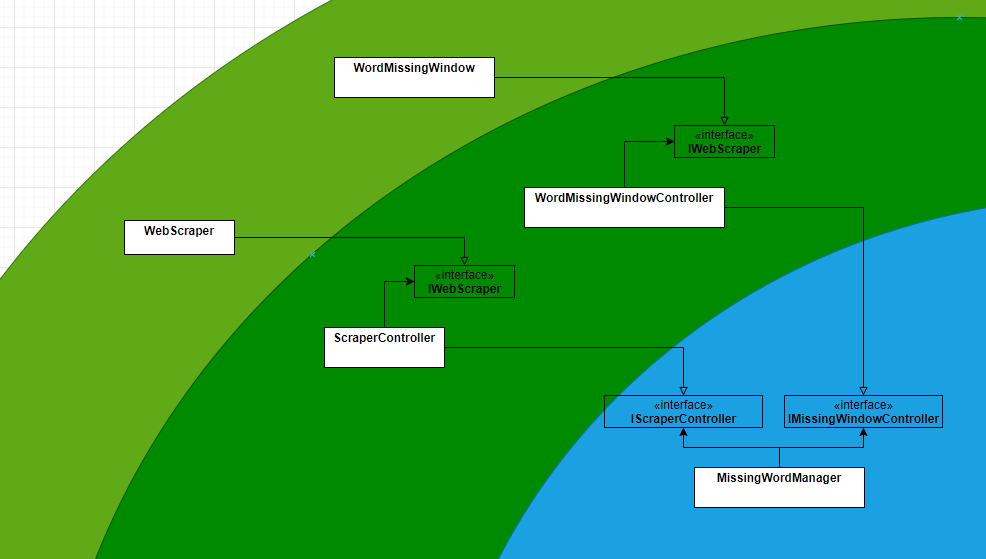
\includegraphics[width=0.8\textwidth]{Bilder/CleanArchitectureWebScraper.PNG}
\caption{\label{Abb:CleanArchitectureWebScraper}Vereinfachtes Klassendiagramm des WebScrapers und zugehöriger GUI}
\end{figure}

\endinput